\documentclass{article}

\usepackage{swiftnav}


\usepackage{draftwatermark, array}
\SetWatermarkLightness{0.9}
\SetWatermarkText{Preliminary}
\SetWatermarkScale{1}
% Suppress numbers from section headings (but preserve PDF TOC).
\makeatletter
\renewcommand\@seccntformat[1]{}
\makeatother
\newcolumntype{$}{>{\global\let\currentrowstyle\relax}}
\newcolumntype{^}{>{\currentrowstyle}}
\newcommand{\rowstyle}[1]{\gdef\currentrowstyle{#1}%
  #1\ignorespaces
}
\newenvironment{mpar}{\par\noindent\minipage{\linewidth}}{\endminipage\par}
%\setlength{\skip\mpfootins}{2cm}
\renewcommand{\thempfootnote}{(\arabic{mpfootnote})}


% ---------------------------------------------------------------------------
\usepackage[section]{placeins}
\version{0.1}
\title{Piksi for UAV Aerial surveying}
\mysubtitle{RTK direct georeferencing with Swift Navigation's Piksi GPS receiver}
\author{Dennis Zollo, Rai Gohalwar}
\date{\today}

\ignorespaces

\begin{document}
\maketitle

\thispagestyle{firstpage}

\section{Abstract}
\label{sec:abstract}
This whitepaper presents using Piksi, a Carrier Phase differential GPS sensor, to georeference aerial images from miocro aerial vehicles (MAVS) for surveying use cases.
It presents both the integration and flight planning methods as well as the surveying  results from flight data as processed by the PIX4D photogrammetry software.
Lastly, the value proposition of using RTK GPS for aerial surveying is evaluated.
\tableofcontents
\newpage
\section{Overview}
\label{sec:Overview}
Due to the impressive capability, low-cost, and increasing popularity of micro aerial vehicles, there is much interest and excitement about the potential applications of the aircraft in the future. One promising application for is aerial surveying for industries such as precision agriculture, mining, and forestry.

In a typical aerial surveying use-case, a fixed wing or mult-rotor aircraft is outfitted with a high-quality camera.  The vehicle overflies the area of interest and captures a series of images which are processed in software to produce Digital Elevation Models (DEM's), Orthomosaics, and 3D point clouds.  These models and deliverables, in turn, can be used for photogammetry applications, volumetric measurements, or crop health measurements which can provide business value for the target use case.

A key part of the data collection process accurate geo-referencing of the photos taken aboard the aircraft.

\section{Equipment and Setup}
\label{sec:equipment}in
here we describe the equipment
\begin{table}[]
\centering
\label{my-label}
\begin{tabular}{|l|c|}
\hline
\multicolumn{2}{|c|}{Vehicle Specifications} \\ \hline
Frame Type            & Quad-Rotor           \\ \hline
Frame                 & Tarot FY650          \\ \hline
Flight Controller     & 3DR Pixhawk          \\ \hline
Motors x 4            & T-Motor MN4006       \\ \hline
Motor Controllers x 4 & X-Rotor 40A OPTO     \\ \hline
Propellers x 4        & Tarot 1555 CF        \\ \hline
Batteries x 2         & Multistar 6S 5200mAh \\ \hline
Weight                & 2942 g               \\ \hline
\end{tabular}
\end{table}
\begin{table}[]
\centering
\label{my-label}
\begin{tabular}{|l|c|}
\hline
\multicolumn{2}{|c|}{Camera Specifications}                                                \\ \hline
Camera                                                                & Sony Nex-5T        \\ \hline
Lens                                                                  & Sony SEL-20F28     \\ \hline
\begin{tabular}[c]{@{}l@{}}Weight\\ (with vehicle mount)\end{tabular} & 424 g              \\ \hline
Sensor                                                                & 16 MP: 4912 x 3264 \\ \hline
\end{tabular}
\end{table}
Camera, focal length, quadcopter
Radios
\section{Method}
\label{sec:method}
Site selection
GCP surveying (skylark)
Mission Planning (mission planner)
Camera setup (exposure, etc)
\section{Post-Processing Techniques}
\begin{figure}
\begin{center}
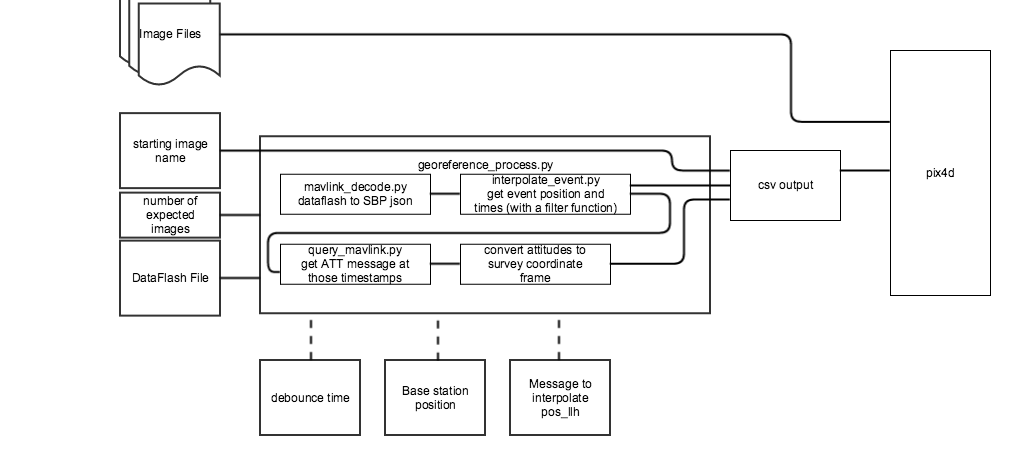
\includegraphics[width=7in]{images/uav_survey_processing_architecture.png}
\end{center}
\end{figure}

\begin{tabular}{l ^ l ^ l ^ l ^ l} \hline
\rowstyle{\bfseries}
Configuration & Description & Pix4D Calibration Method & GPS Sensor & Ground Control \\ \hline
\rowstyle{}
A & Piksi RTK Std & Standard & Piksi RTK (Fixed) & None  \\ \hline
B& Piksi RTK Std & Standard & Piksi RTK (Fixed) & 7 GCPS  \\ \hline
C & Piksi RTK Acc & Accurate & Piksi RTK (Fixed) & None  \\ \hline
D & Piksi RTK Acc & Accurate & Piksi RTK (Fixed) & 7 GCPS  \\ \hline
E & Ublox STD & Standard & UBLOX & None  \\ \hline
F & Ublox STD & Standard & UBLOX & 7 GCPS  \\ \hline
G & Ublox Acc & Accurate & UBLOX & None  \\ \hline
H & Ublox Acc & Accurate & UBLOX & 7 GCPS  \\ \hline
\end{tabular}
\thispagestyle{lastpage}
\end{document}
